\chapter{Implémentation}
\section{Formation sur Unity}
Afin de se familiariser avec Unity, car il n'en avait aucune connaissance avant le début de ce projet, l'étudiant a suivi deux tutoriels disponibles
sur le site du logiciel\cite{UnityEssentialsPathway}\Cite{MobileARDevelopment}. Le premier est \textit{Unity Essentials}, il présente :

\begin{itemize}[label={\textbullet}]
    \item L'installation d'Unity
    \item La création de projet avec ou sans template.
    \item Une explication de l'interface de l'éditeur d'Unity ainsi que ses commandes principales.
    \item Une introduction aux environnement 2D et 3D.
    \item Une introduction à l'ajout d'audio.
    \item Une introduction à la programmation (scripts).
    \item Le déploiement sur WebGL d'une application.
\end{itemize}


Le deuxième tutoriel est spécifique à la réalité augmentée, \textit{Mobile AR Development} et explique comment :

\begin{itemize}[label={\textbullet}]
    \item Créer un filtre pour visage (comme Snapchat par exemple).
    \item Détecteur un repère (QR Code, autre) puis faire apparaître un objet dessus.
    \item Détecter un plan en RA, puis faire apparaître un objet en cliquant sur l'écran du téléphone.
    \item Déployer une application sur smartphone.
\end{itemize}
\newpage
\section{Implémentation de l'application}
\subsection{Déploiement de Geospatial Creator dans Unity}
Pour avoir accès à Geospatial Creator dans Unity, un tutorial est fourni par Google\cite{GetStartedGeospatial}. Les étapes importantes sont :
\begin{itemize}[label=\textbullet]
    \item Suivre le lien sur la page qui redirige vers "Getting started with ARCore Extensions for AR Foundation"
    \item Installer les Package ARCore Extensions (attention à la version d'ARFoundation) et Cesium
    \item Revenir sur la page principale
    \item Autoriser les différentes API dans la console Google Cloud et récupérer la clé d'API (cette étape sera mieux décrite dans le rapport final)
    \item Importer le projet d'exemple de ARCore Extensions du Package Manager d'Unity
    \item Activer Geospatial et Geospatial Creator dans Edit -> Project Settings -> XR Plug-in Management -> ARCore Extensions et ensuite insérer la clé d'API dans ce menu.
\end{itemize}
\subsection{Test de l'application d'exemple de Google}
Une fois \acrshort{ggc} déployé dans Unity, la scène d'exemple peut être ouverte dans l'éditeur :
\begin{figure}[H]
    \centering
    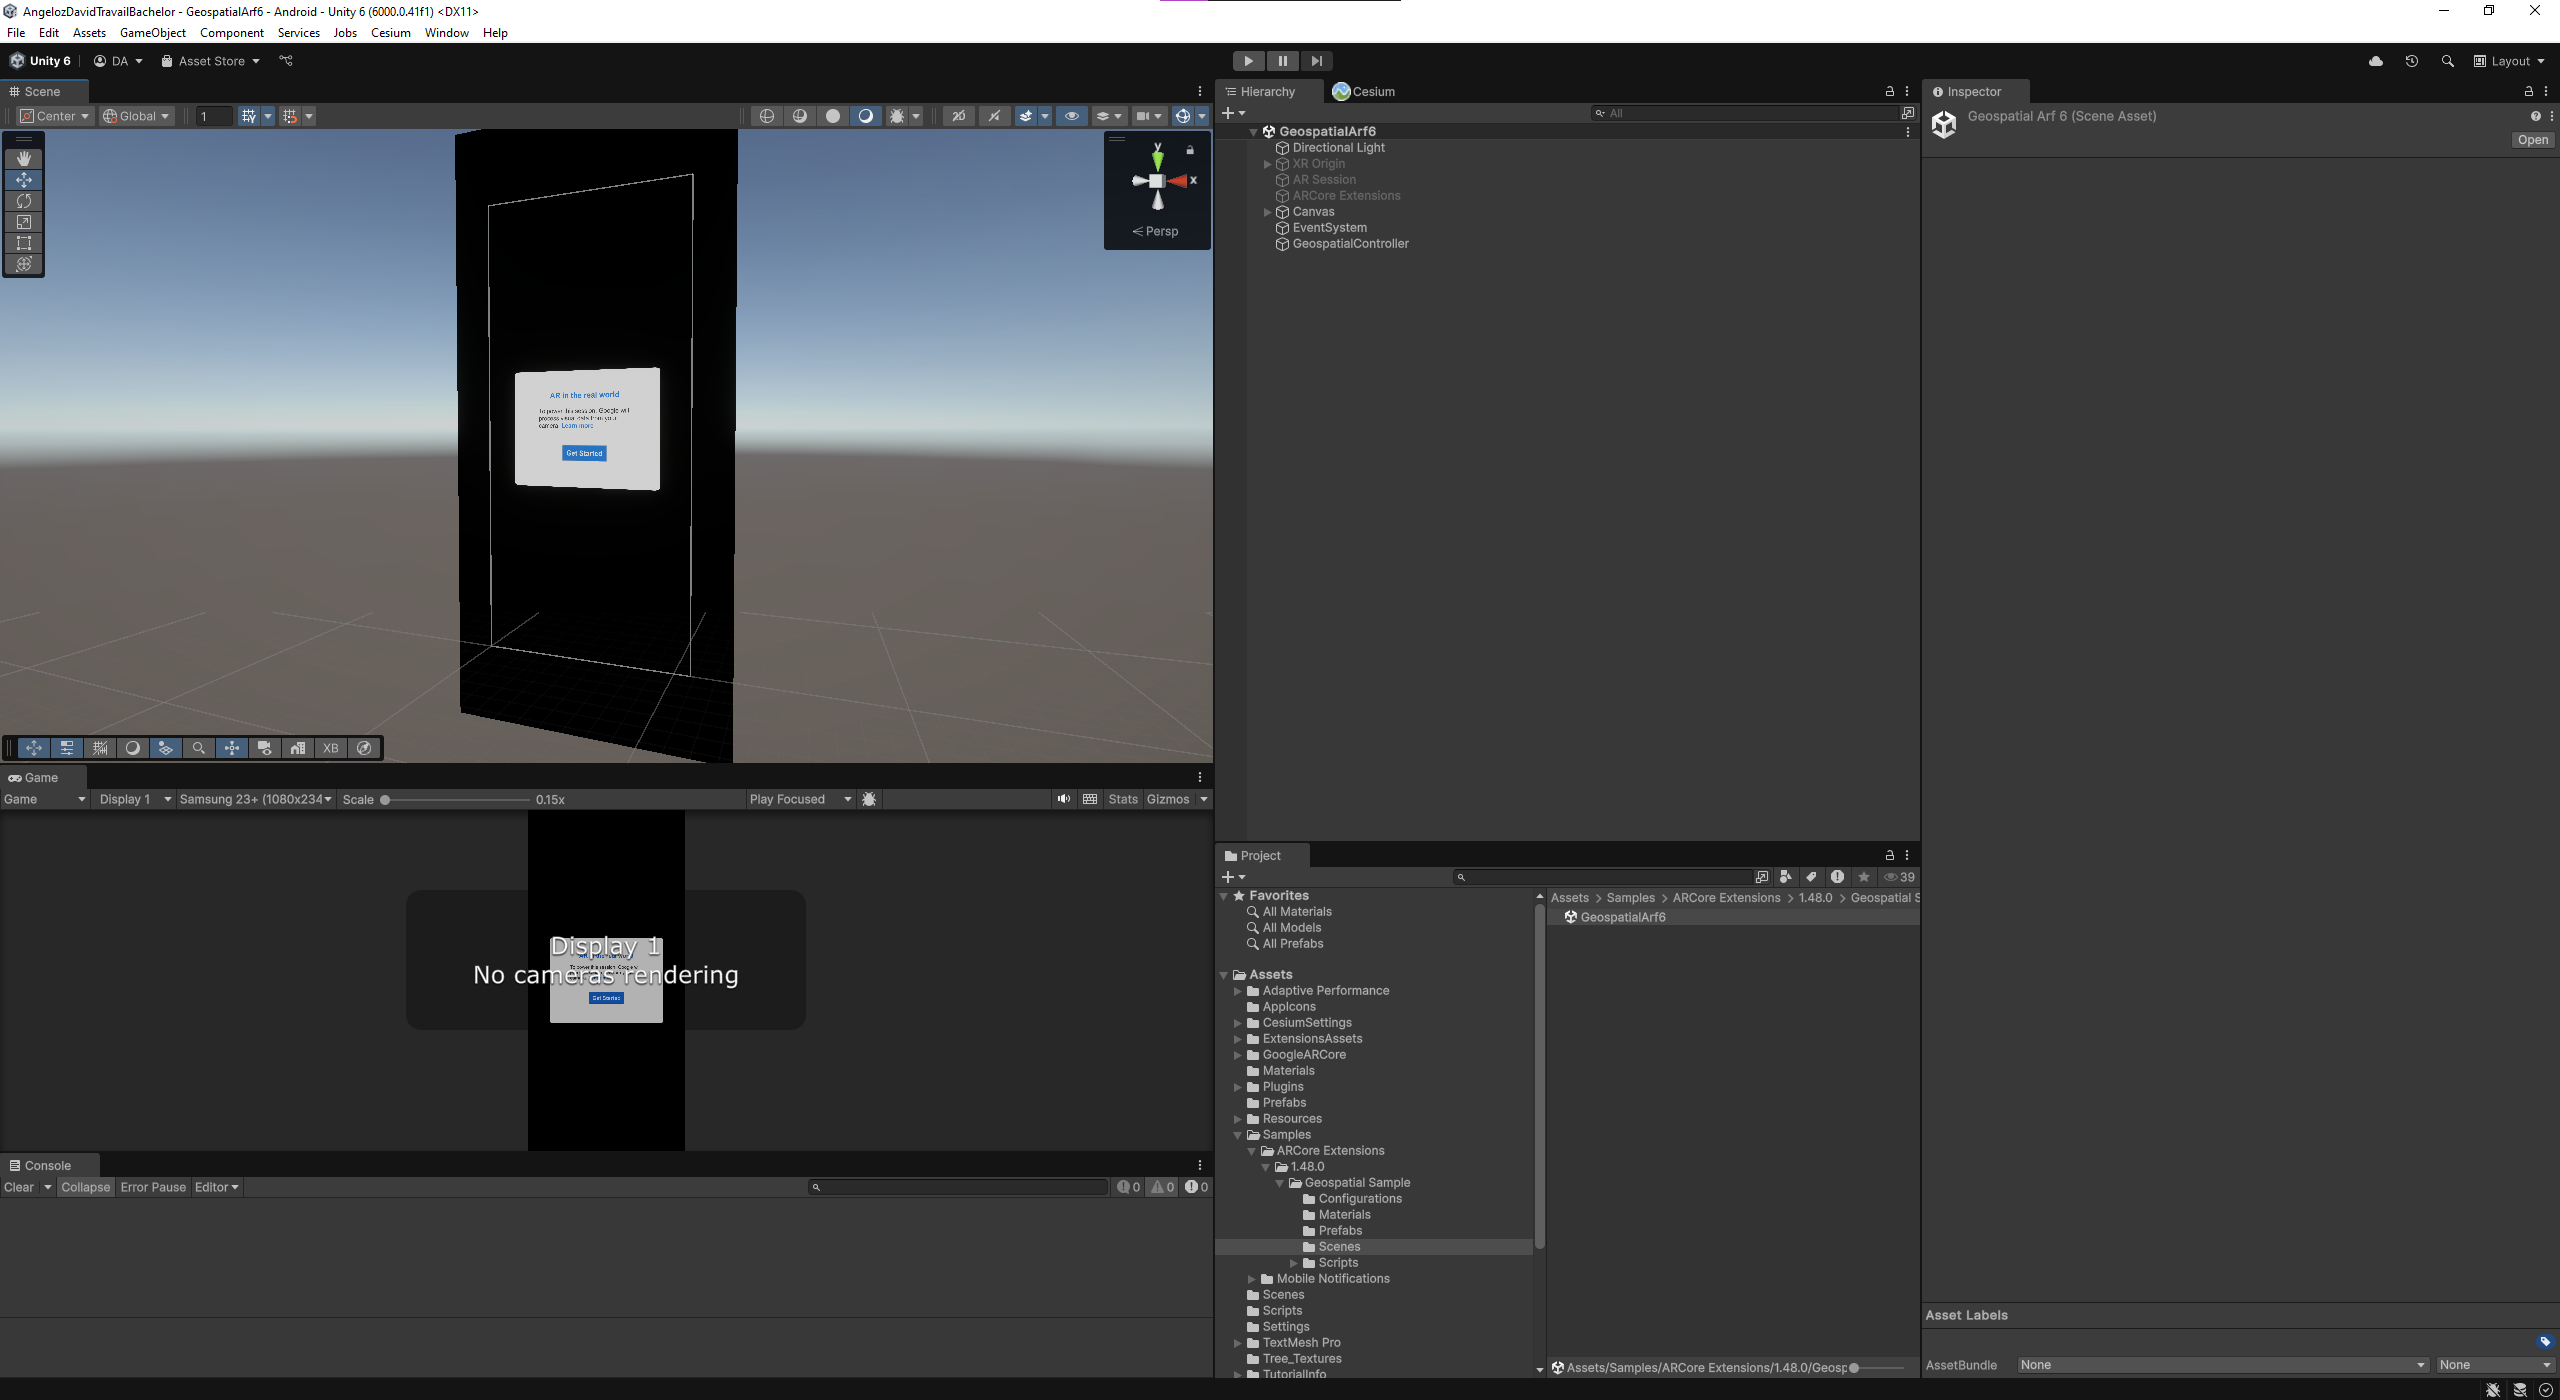
\includegraphics[width=1\linewidth]{assets/figures/Screenshots/GGC_1.png}
    \caption{Editeur Unity, example de Geospatial Creator ouvert.}
    \label{fig:GGC_1}
\end{figure}
L'arborescence dans l'onglet Project montre oû est située la scène d'exemple.


Il faut ensuite créer un objet \textbf{Geospatial Creator Origin} :
\begin{figure}[H]
    \centering
    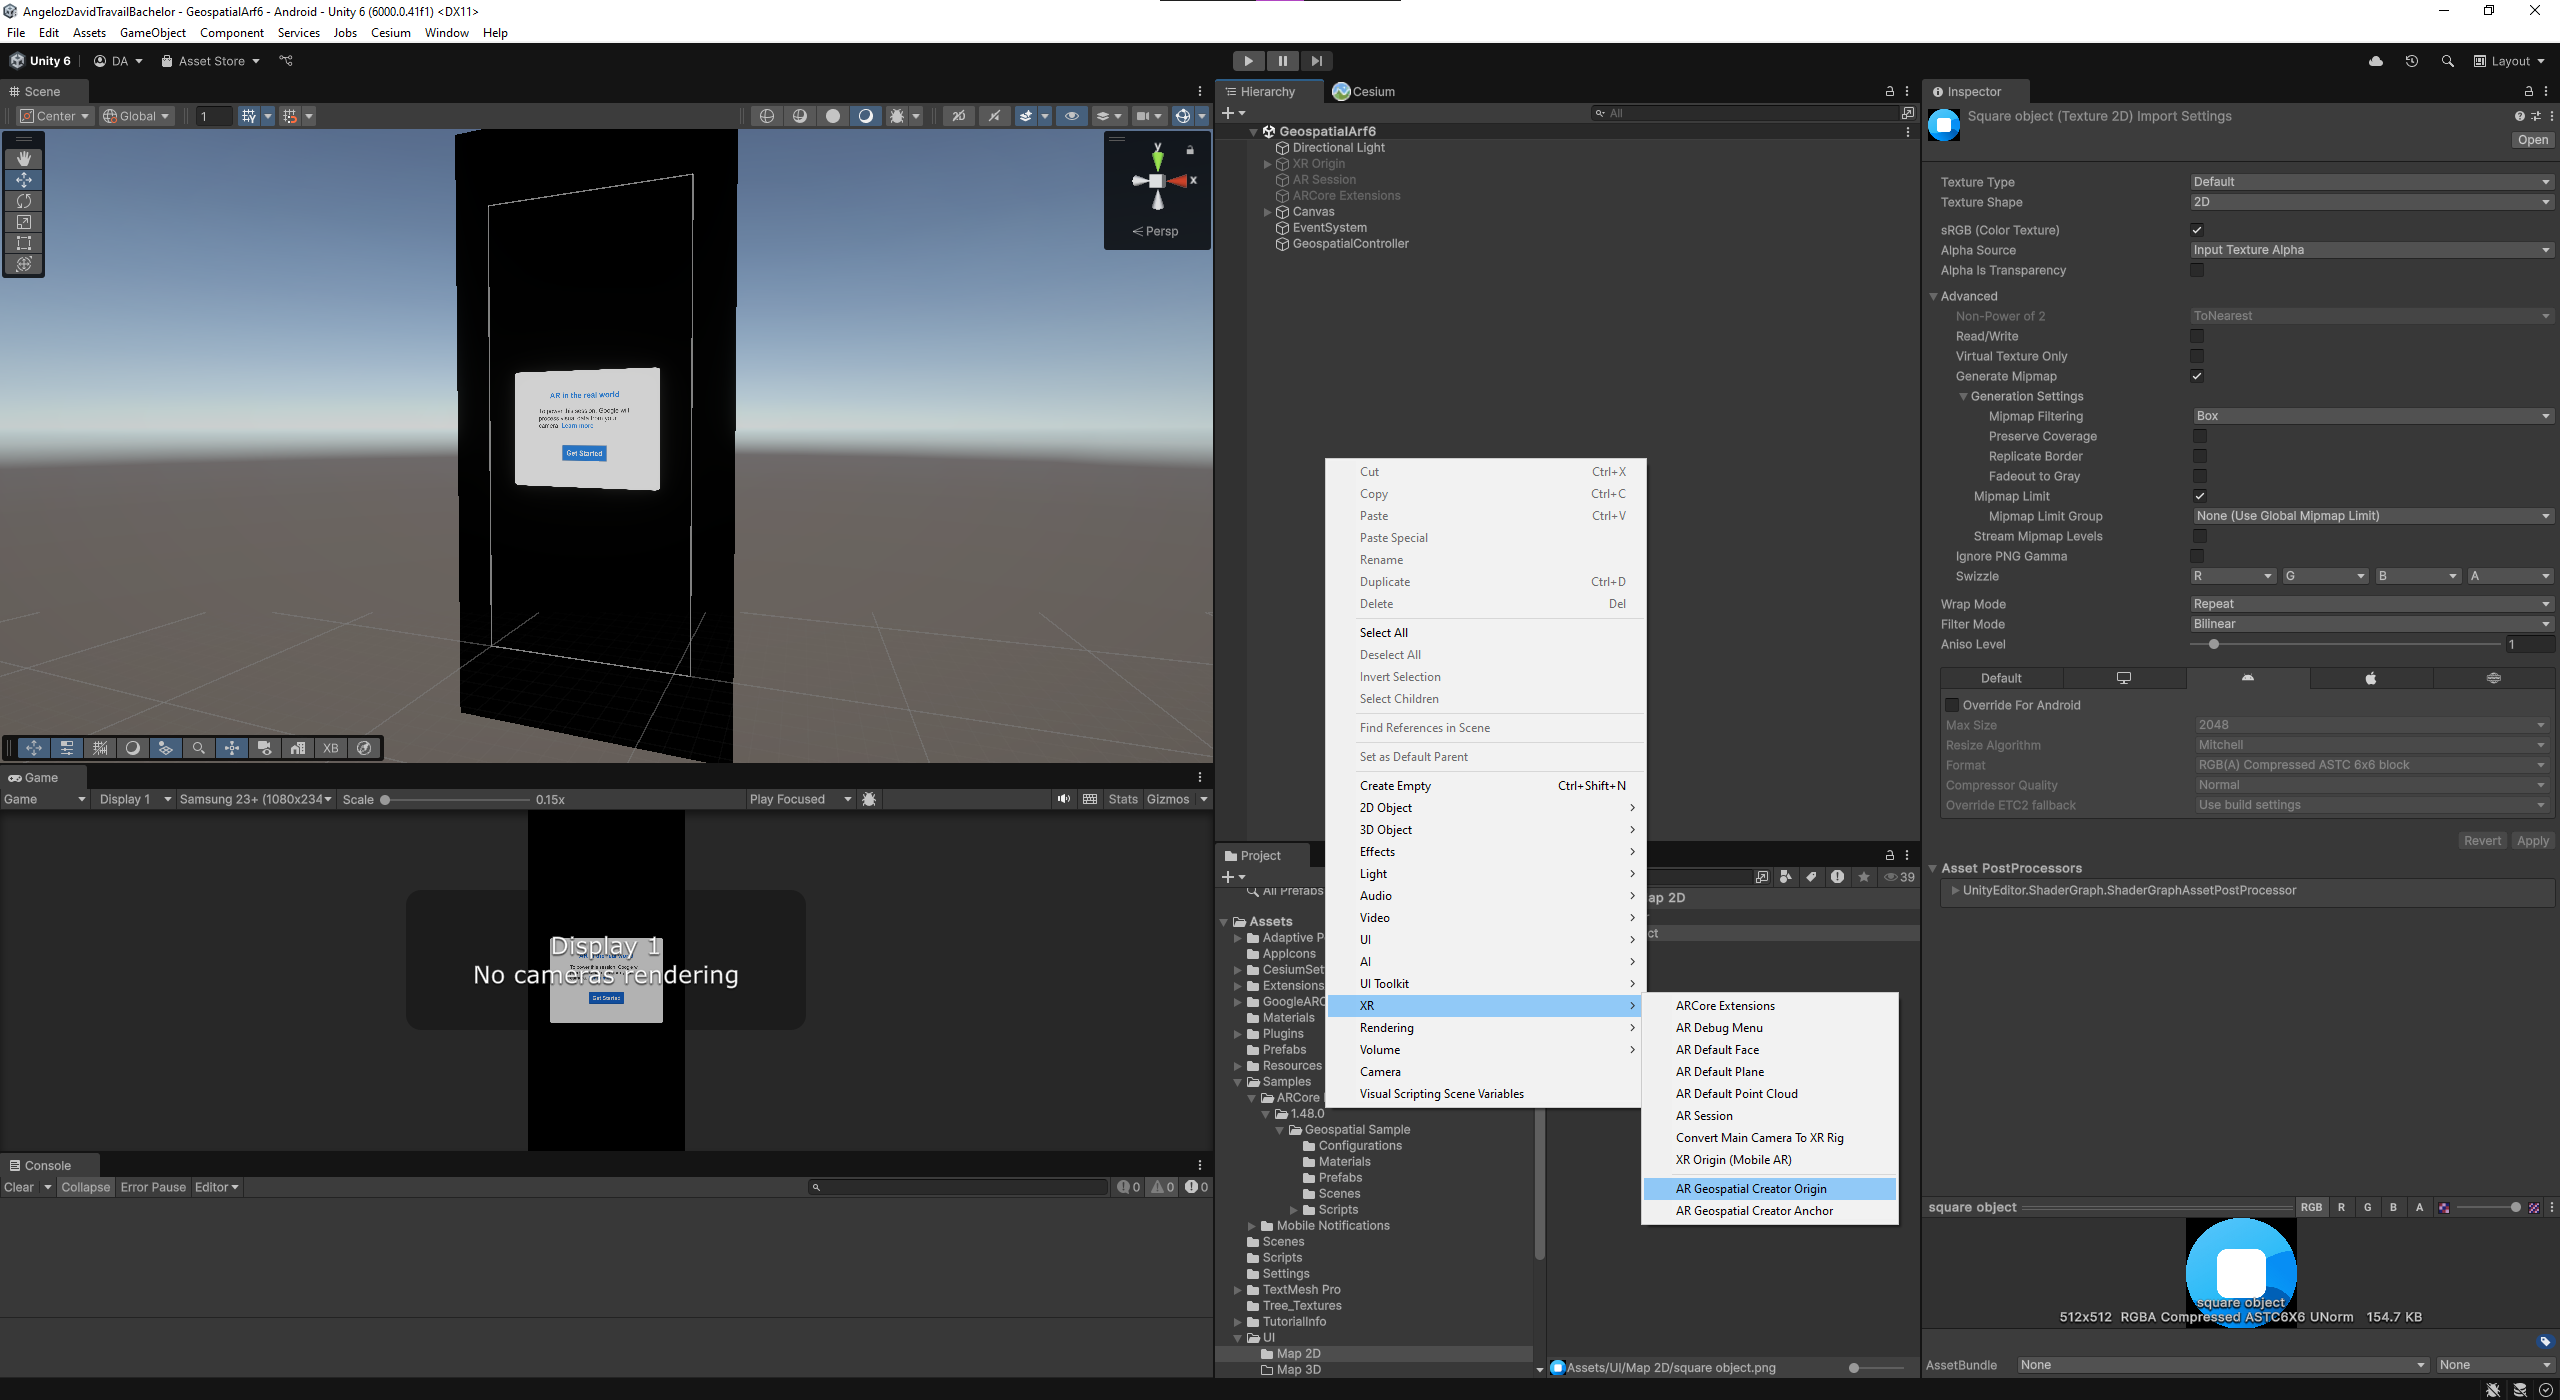
\includegraphics[width=1\linewidth]{assets/figures/Screenshots/GGC_2.png}
    \caption{Editeur Unity, création de l'objet Geospatial Creator Origin.}
    \label{fig:GGC_2}
\end{figure}

La dernière étape pour faire fonctionner le projet d'exemple est de faire fonctionner Cesium :

\begin{figure}[H]
    \centering
    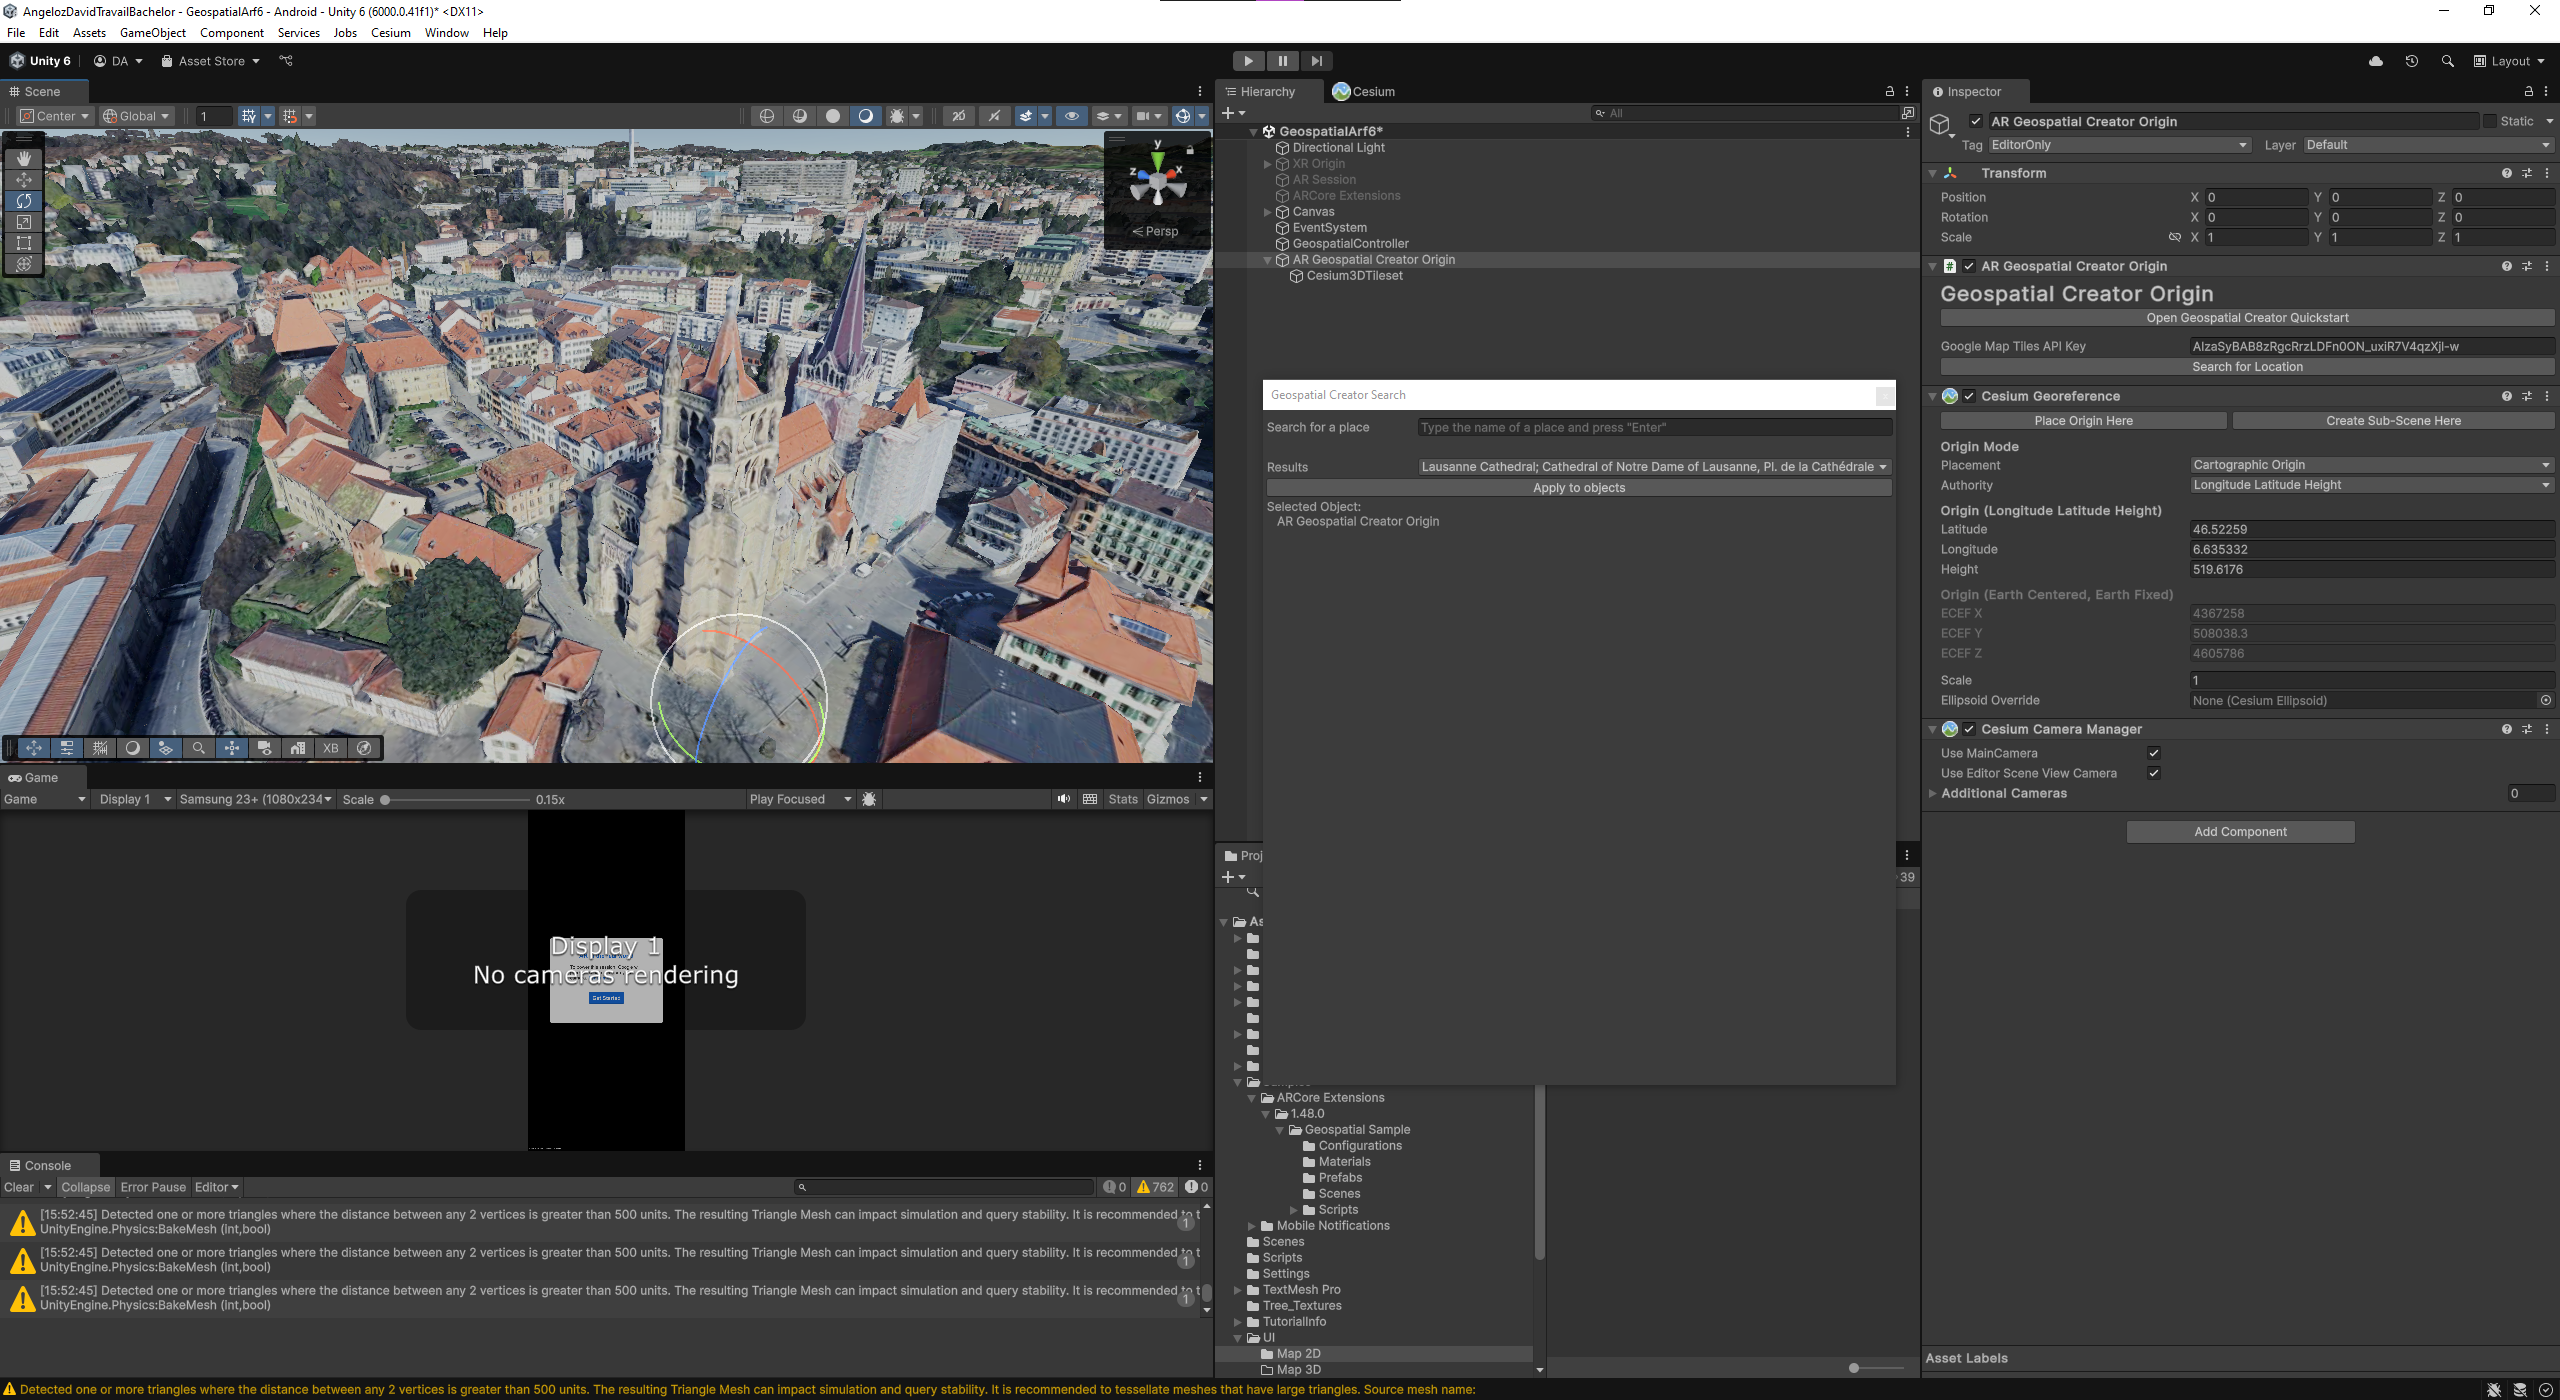
\includegraphics[width=1\linewidth]{assets/figures/Screenshots/GGC_5.png}
    \caption{Editeur Unity, Activation de Cesium et emplacement de l'origine.}
    \label{fig:GGC_5}
\end{figure}

Dans la figure ci-dessus, l'utilisateur a déjà cliqué sur le bouton \textbf{Add Cesium Georeference Component} et inséré sa clé d'API dans le champ correspondant.

Le bouton \textbf{Search for Location} ouvre la petite fenêtre sur la capture d'écran qui permet de chercher un lieu dans le monde. En appuyant sur le bouton \textbf{Apply to objects}
les textures et les volumes sont appliqués et l'origine est changée d'emplacement.
Ici, la cathédrale de Lausanne a été choisie comme exemple. Dans l'onglet Scene on peut la voir ainsi que ses environs en 3D et avec les bonnes textures.

Note : La HEIG-VD avait été choisie comme exemple. Cependant, il semble que toute la ville d'Yverdon-les-Bains et ses environs ne possèdent pas encore
de données qui permettent à GGC de les modéliser en 3D. Le site de Cheseaux apparaît donc plat et on pourrait tout de même travailler avec
en testant plus rigoureusement les placements d'objets.

\subsection{Ajout d'un objet virtuel proche de l'origine}
En revenant à l'origine, soit proche d'où habite l'étudiant et comme pour la création de l'objet \textbf{Geospatial Creator Origin}, on crée un \textbf{Geospatial Creator Anchor} auquel on vient ajouter un objet enfant
qui est un simple cube avec un \textit{material} de couleur rouge et un script  qui permet de faire tourner l'objet sur lui-même (ces deux propriétés sont visibles dans l'onglet Inspector)

\begin{figure}[H]
    \centering
    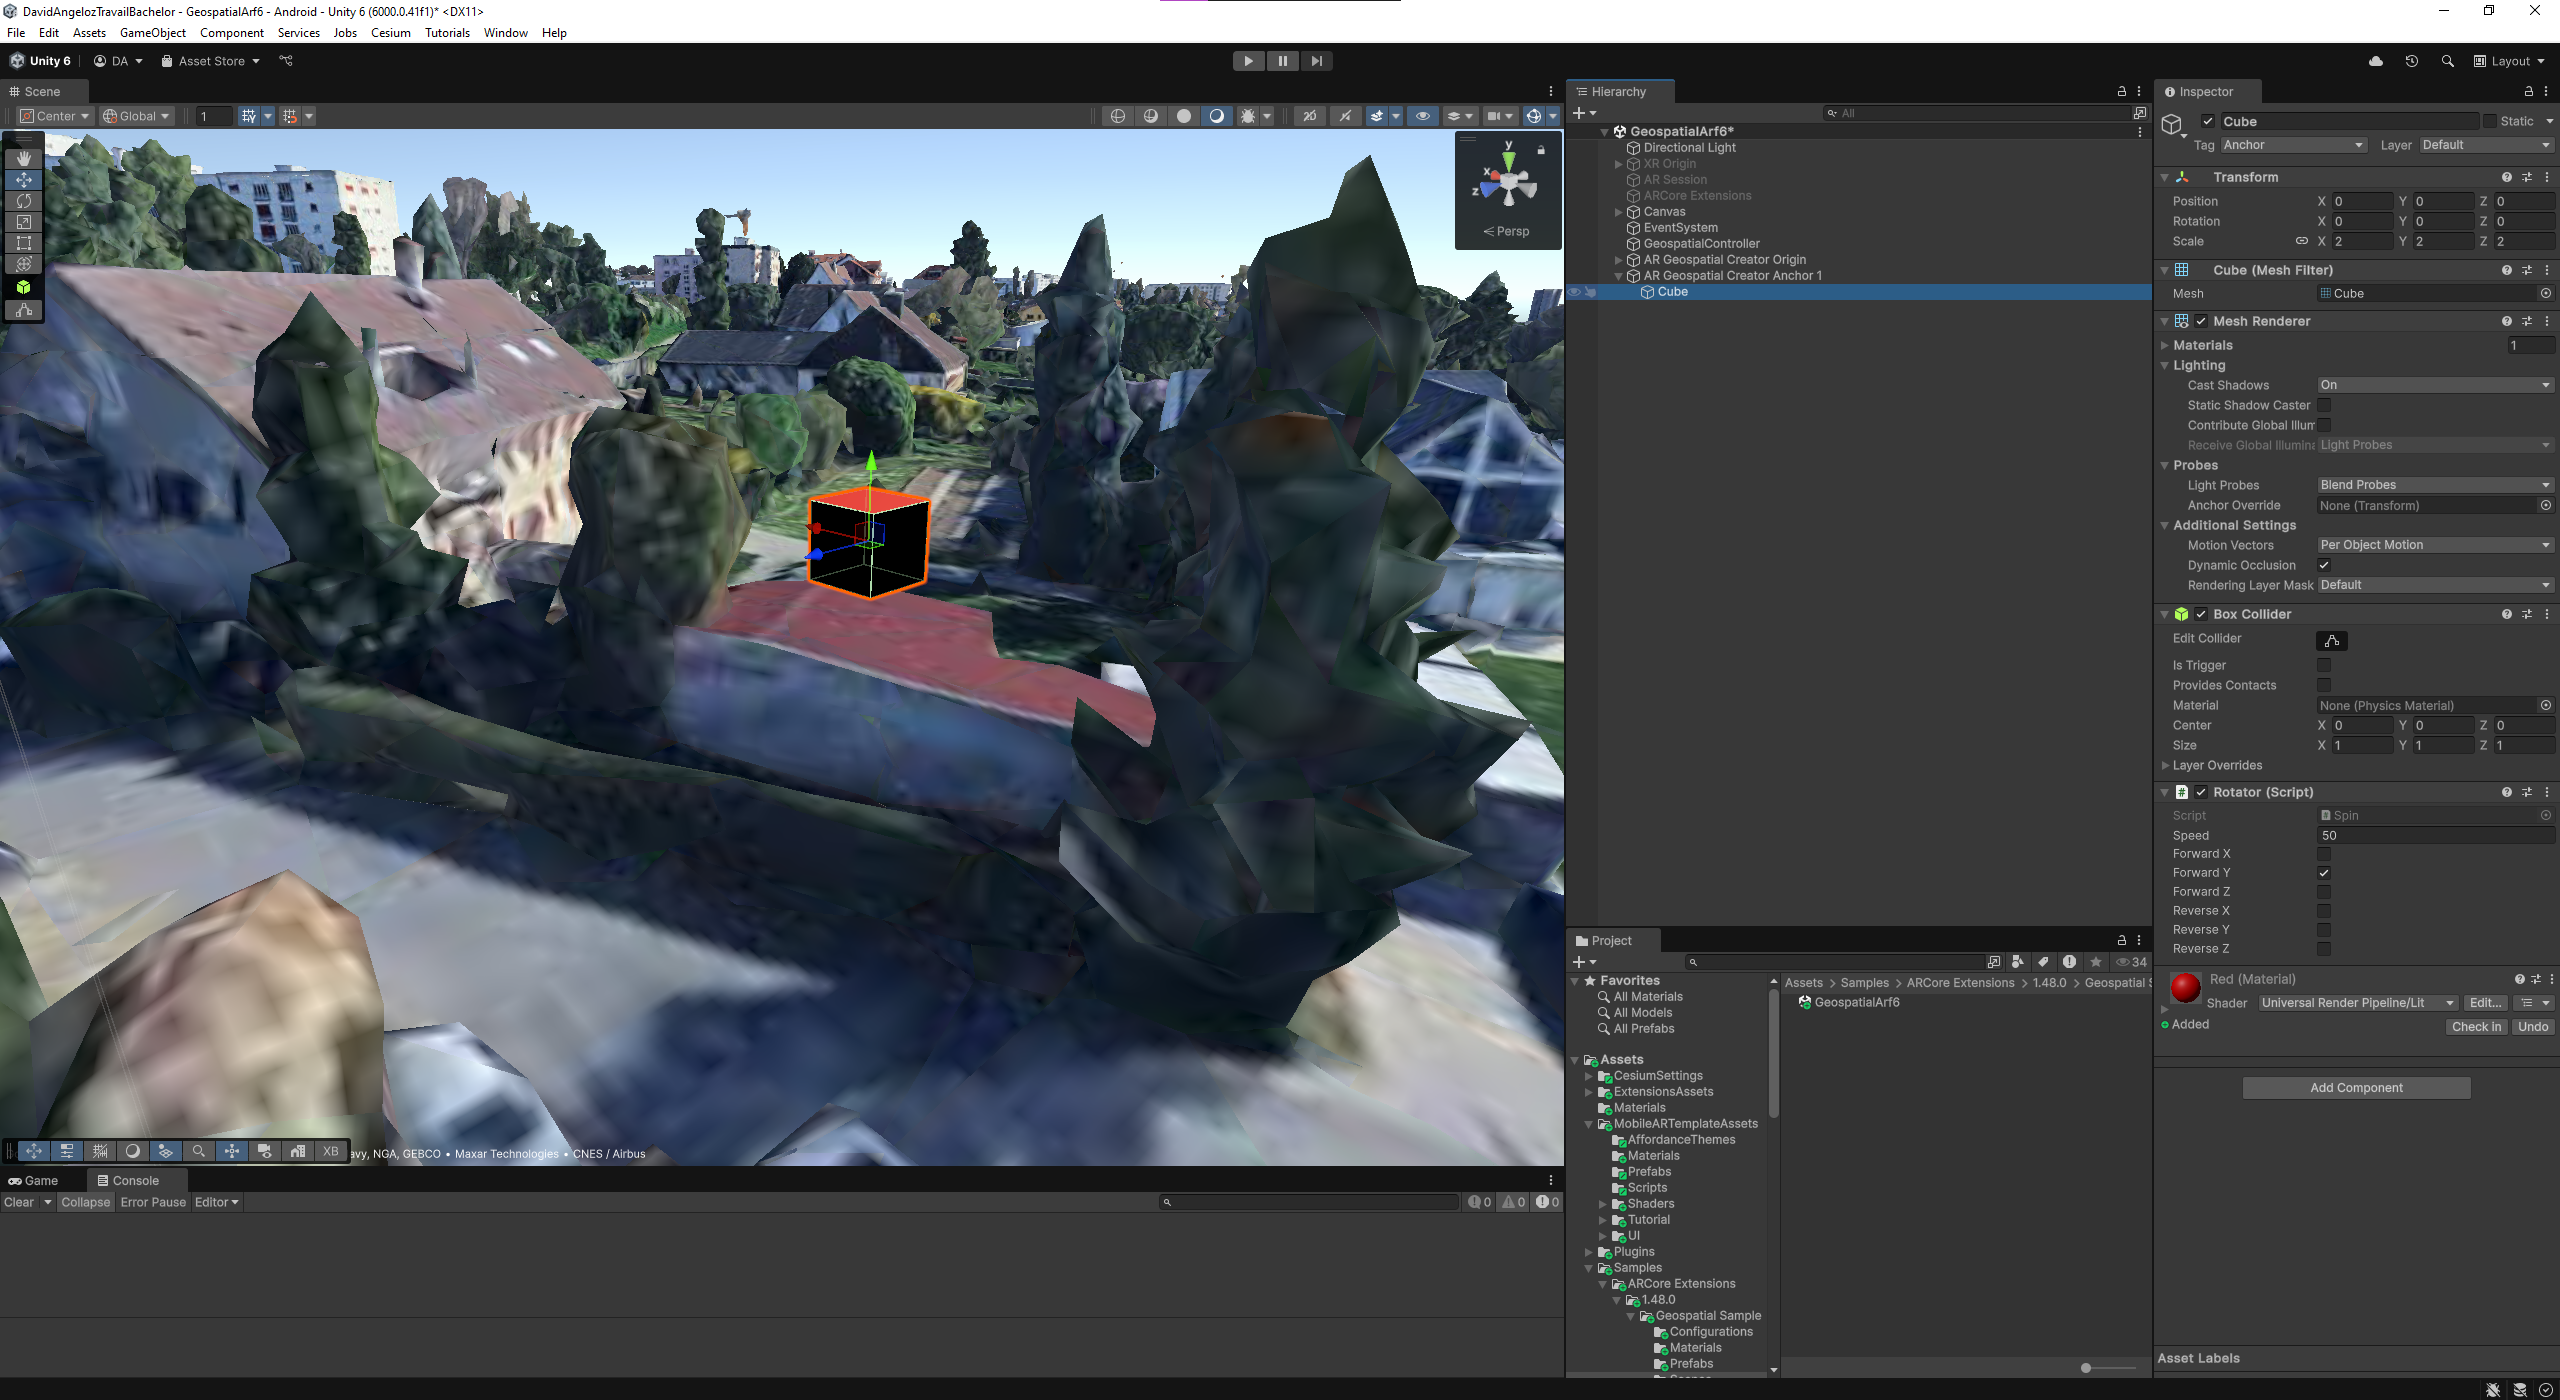
\includegraphics[width=1\linewidth]{assets/figures/Screenshots/GGC_3.png}
    \caption{Editeur Unity, Ajout d'un objet virtuel avec une anchor.}
    \label{fig:GGC_3}
\end{figure}
Une fois l'application téléchargée sur téléphone. On peut pointer la caméra du smartphone vers le petit bâtiment qu'on reconnaît de Unity et le cube apparaît.
Un autre point important auquel il faut faire attention sans les anchor qu'on peut générer en cliquant sur l'écran, elles sont au nombre de quatre et son visible sur la route. C'est à partir de cette méthode (le raycasting)
qu'on va pouvoir interagir avec les objets virtuels.

\begin{figure}[H]
    \centering
    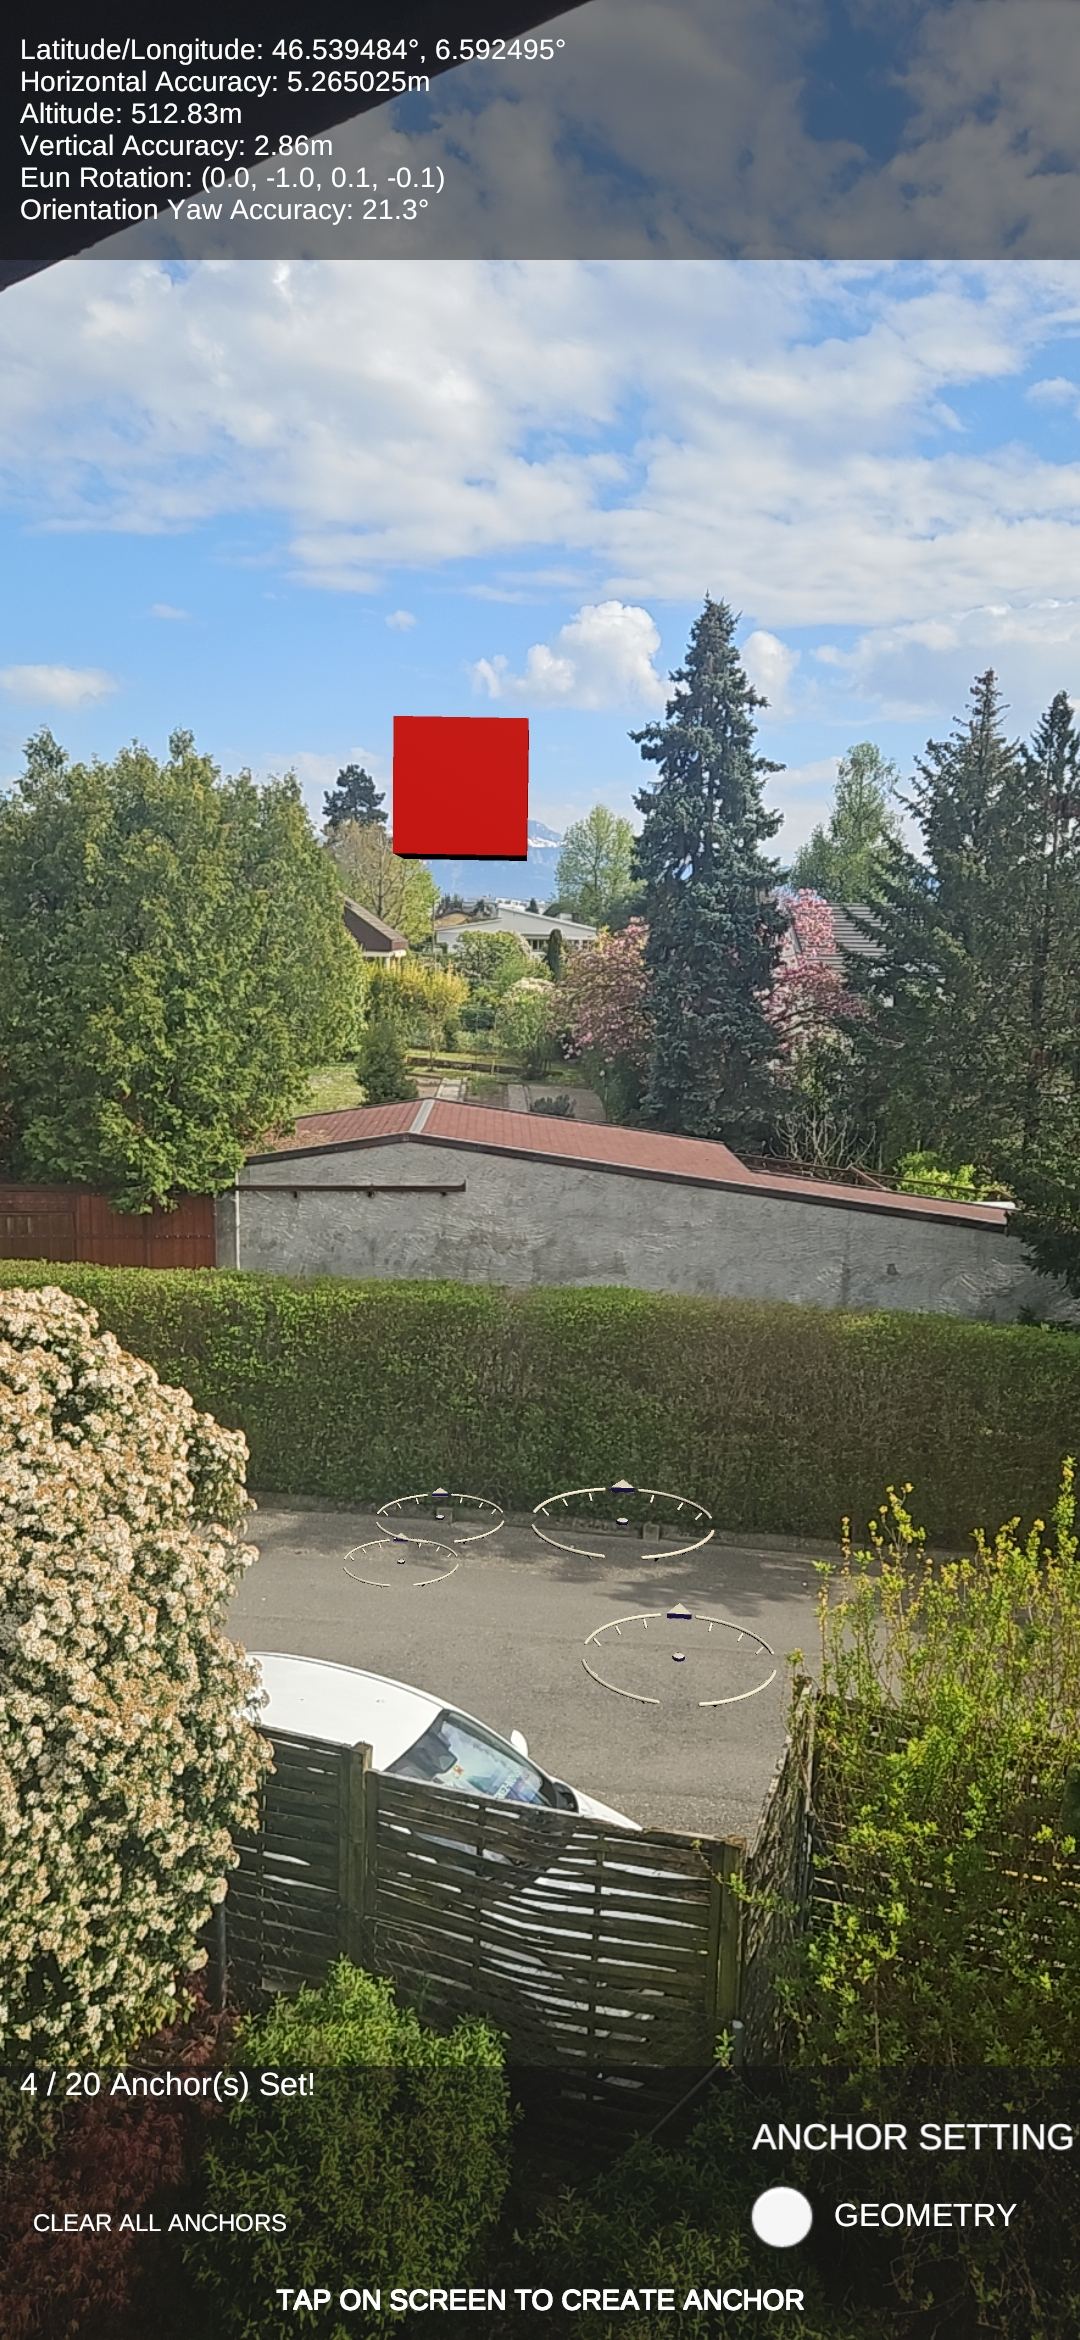
\includegraphics[width=0.5\linewidth]{assets/figures/Screenshots/geospatial example.jpg}
    \caption{Vue de l'objet virtuel ajouté depuis le smartphone.}
    \label{fig:GeoSample}
\end{figure}

\subsection{Interaction avec l'objet}
Au moment de l'écriture du rapport, l'objet affiché le joueur ou la joueuse ne peut pas encore avoir d'interaction avec les objets affichés.
\subsection{Choix du parcours}
Pour avoir un parcours qui se place dans du concret, les transports lausannois
ont été contactés dans le but de leur proposer une collaboration, l'étudiant ayant pensé à
utiliser un parcours, qui fait se déplacer l'utilisateur dans toute la ville de Lausanne,
créé en 2021 pour les 125 ans des tl.\cite{hatetVeriteLionsLausannois2021} Malheureusement, aucune réponse n'a été reçue de leur
part pour l'instant.

Un parcours alternatif est créé par l'étudiant pour palier l'absence de
cette collaboration. Il consiste en quelques objets virtuels qui seront placés dans un parc proche d'où il habite.

\subsection{Affichage d'une carte style Google Maps}
Dans le futur, et pour que l'utilisateur puisse se déplacer comme s'il utilisait une application comme
Google Maps, le but serait d'implémenter une carte en 2D avec l'emplacement du joueur ou de la joueuse ainsi que l'emplacement
des objets virtuels à atteindre. Encore une fois la cathédrale de Lausanne est prise comme exemple, pour montrer sur une maquette à quoi
devrait ressembler la vue sur smartphone. Le rond bleu est l'emplacement du joueur et les ronds avec un carré à l'intéieur sont les objets
virtuels.

\begin{figure}[H]
    \centering
    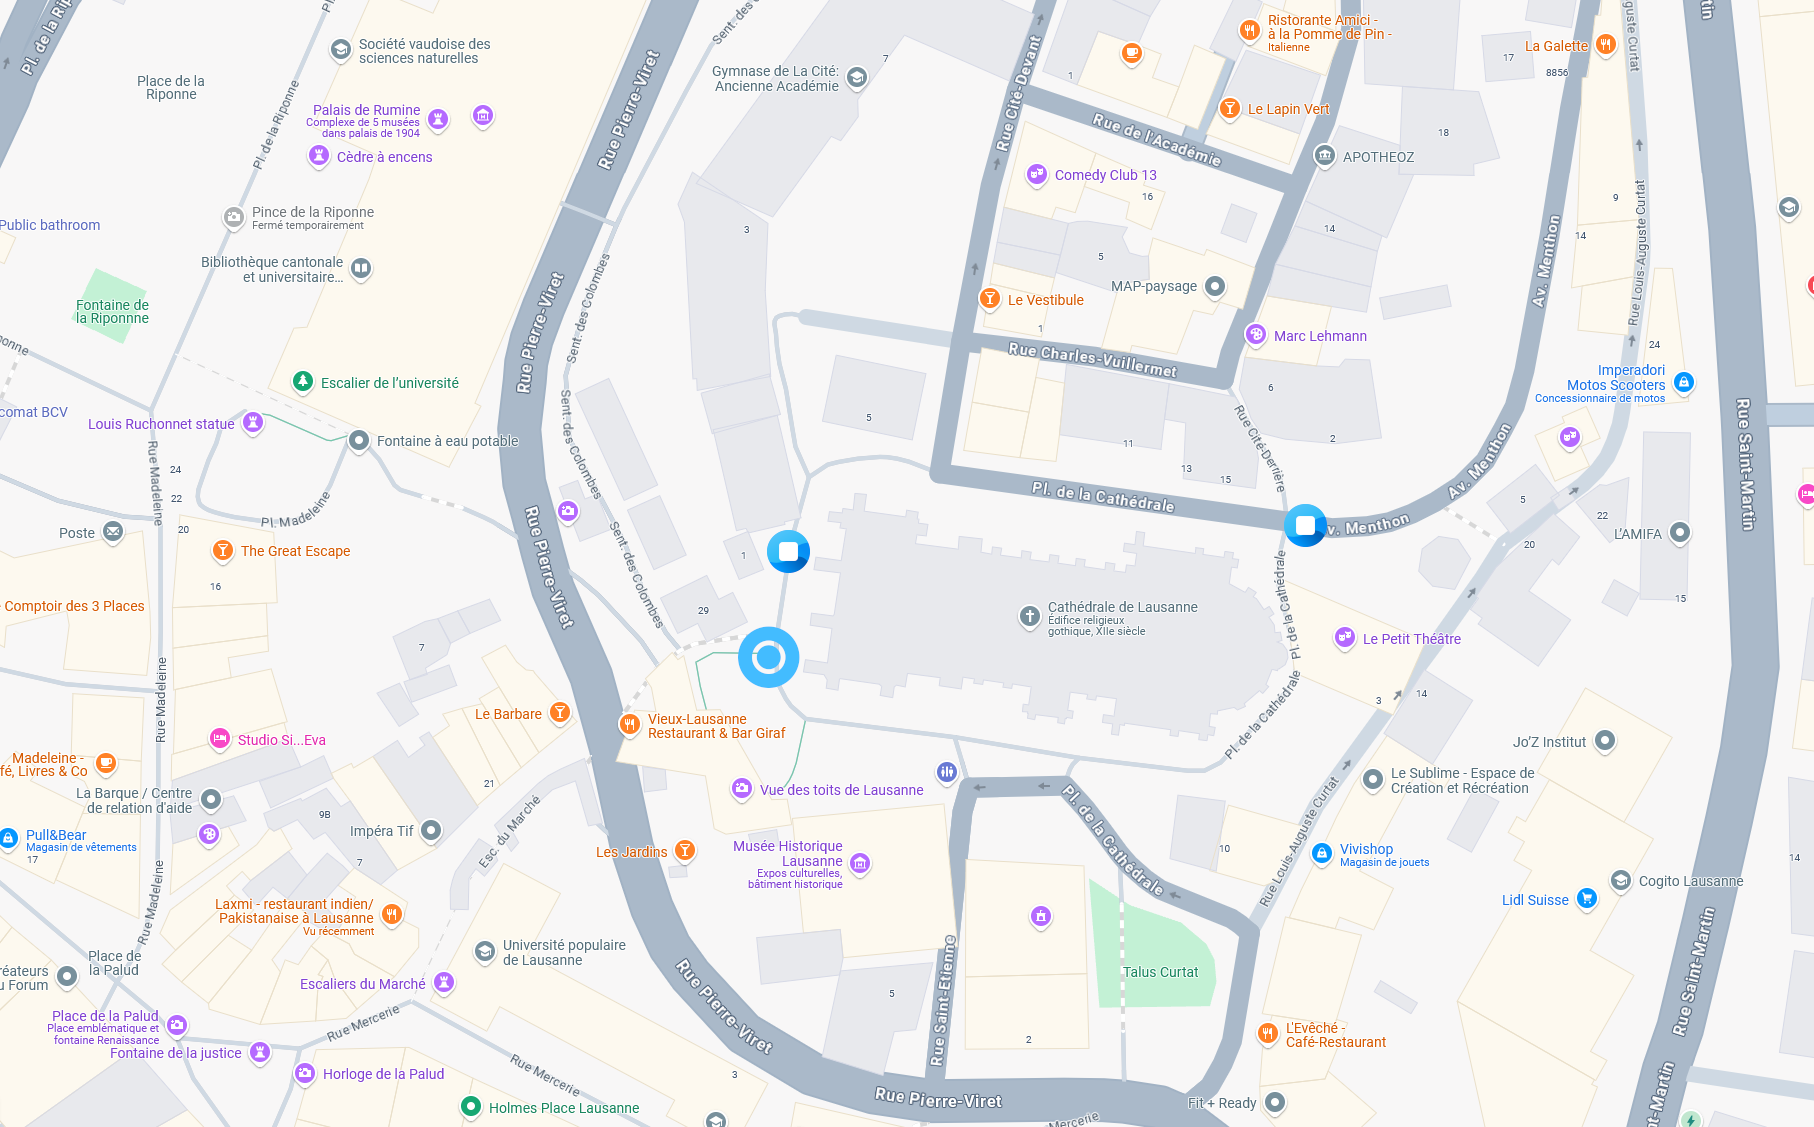
\includegraphics[width=1\linewidth]{assets/figures/Screenshots/Maps.png}
    \caption{Maquette de la vue en 2D, avec indicateurs de joueur et d'objets.}
    \label{fig:Maps}
\end{figure}
% Ce chapitre est consacré à la description détaillée de l'implémentation de votre projet. Il a pour objectif d'expliquer, de manière claire et méthodique, comment vous avez concrètement mis en œuvre votre travail. Vous y présenterez, étape par étape, le processus qui a conduit à la réalisation de votre projet, en justifiant les choix techniques et méthodologiques effectués.

% \index{expérience}
% Vous devez décrire le déroulement de vos expériences, en précisant le cadre dans lequel elles ont été menées ainsi que les outils et technologies utilisés. Ce chapitre doit permettre au lecteur de comprendre non seulement ce que vous avez fait, mais aussi pourquoi vous avez opté pour cette approche.

% Exposez de manière structurée la conception globale de votre projet en illustrant vos explications par des schémas, des diagrammes ou des modèles visuels -- tels que des diagrammes de classes, de flux ou des organigrammes -- afin de clarifier votre démarche.

% Que ce soit pour une architecture logicielle, une conception électronique ou une analyse de données, chaque aspect de votre travail doit être présenté de façon logique et détaillée. Il est essentiel de justifier vos choix en soulignant leur pertinence au regard des objectifs fixés et de la problématique posée.

% Vous êtes libre de structurer ce chapitre en plusieurs sections distinctes, en fonction de la nature de votre projet. L'objectif est d'offrir au lecteur une vision claire de la manière dont vous avez développé votre travail, en mettant en lumière non seulement les actions entreprises, mais également les décisions qui les ont motivées. Votre implémentation doit refléter une réflexion méthodique et rigoureuse, guidée par la problématique et les objectifs initiaux.
